\documentclass[letterpaper, 12pt]{article}
\usepackage{amsmath}
\usepackage[margin=1in]{geometry}
\usepackage{adjustbox}
\usepackage{graphicx}
\usepackage[final]{pdfpages}
\usepackage{bm}
\usepackage{sectsty}
\usepackage{titlesec}
\usepackage{lipsum}
\usepackage{subcaption}
\usepackage{listings}
\usepackage{pgffor}
\usepackage{rotating}
\usepackage{xcolor}  
\usepackage{amsthm}
\usepackage{csvsimple}
\usepackage{enumitem}
\usepackage{amssymb} 
\usepackage{amsfonts}
\usepackage{tikz}
\usepackage{tikz-3dplot}
% \setlength{\tabcolsep}{0.5cm} 
\newcommand{\thickhat}[1]{\mathbf{\hat{\text{$#1$}}}}
\renewcommand{\lstlistingname}{Program}

\newtheoremstyle{custom}
  {3pt}
  {3pt}
  {\itshape}
  {} 
  {\bfseries}
  {. }  
  { }   
  {\thmname{#1} \thmnumber{#2} \thmnote{ #3}}

\theoremstyle{custom}


\newtheorem{definition}{Definition}
% \newtheorem{theorem}{Theorem}
\newtheorem*{theorem}{Theorem}
\sectionfont{\fontsize{12}{15}\selectfont}
\titleformat{\section}
{\normalfont\normalsize\bfseries}
{(\thesection)}{1em}{}

\title{Cauchy's Integral Formula}
\author{Masaru Sawata}
\begin{document}

\maketitle
\begin{theorem}[Cauchy's Integral Formula]
\end{theorem}
If a complex-valued function $f: \mathbb{C} \rightarrow \mathbb{C}$ is analytic at any point in a domain $\Omega$ closed by the contour $C$,
\begin{equation*}
  \frac{1}{2\pi i}\oint_C \frac{f(z)}{z - z_0} \, dz = f(z_0)
\end{equation*}\\

\begin{proof}
  Since $f$ is an analytic function in a domain $\Omega$, 
  $\displaystyle \frac{f(z)}{z - z_0}$ is analytic except $z = z_0$.
  Applying the Cauchy's Integral Theorem to the integral along the contour shown in Figure \ref{fig3}, 
  \begin{equation*}
    \oint_C \frac{f(z)}{z - z_0} \, dz + \oint_{-C^\prime} \frac{f(z)}{z - z_0} \, dz = 0
  \end{equation*}
  where $-C^\prime$ is the curve $C^\prime$ traversed in the oposite direction. Thus,
  \begin{equation*}
    \oint_C \frac{f(z)}{z - z_0} \, dz - \oint_{C^\prime} \frac{f(z)}{z - z_0} \, dz = 0
  \end{equation*}
  \begin{equation*}
    \oint_C \frac{f(z)}{z - z_0} \, dz = \oint_{C^\prime} \frac{f(z)}{z - z_0} \, dz
  \end{equation*}


  \begin{figure}[htbp]
    \centering
    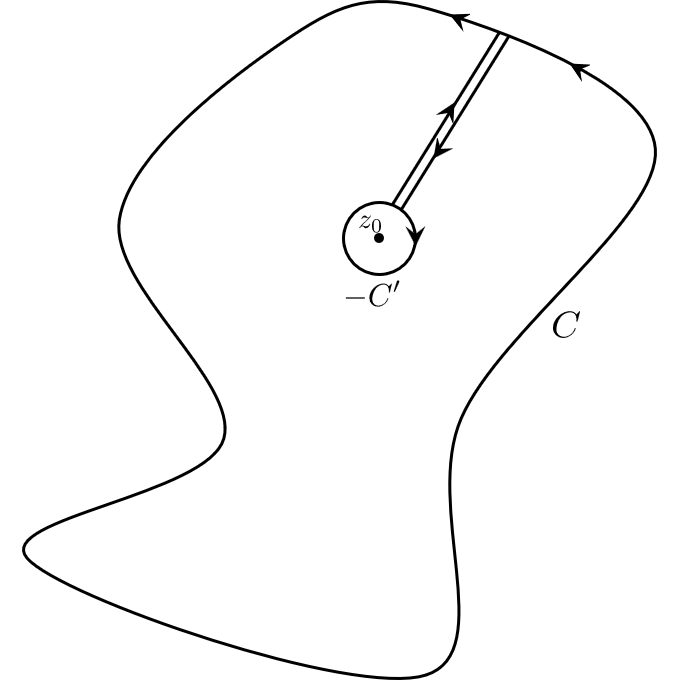
\includegraphics[width=.5\columnwidth]{Contour3.png}
    \caption{Contour for integration}
    \label{fig3}
  \end{figure}

  Therefore, we can use the smaller contour to evaluate the integral.
  Let $C^\prime$ be the circle whose radius is $r$ centered at $z_0$. As mentioned earlier, the integral does not change by $r$ as long as $C^\prime$ is in the $C$.
  Then,
  \begin{align*}
    \oint_C \frac{f(z)}{z - z_0} \, dz 
    &= \oint_{C^\prime} \frac{f(z)}{z - z_0} \, dz \\
    &= \int_{0}^{2\pi} \frac{f(z_0 + re^{i\theta})}{z_0 + re^{i\theta} - z_0} ire^{i\theta}\, d\theta \\
    &= i\int_{0}^{2\pi} f(z_0 + re^{i\theta}) \, d\theta
  \end{align*}
  Since $f$ is an analytic function, it is continuous at $z = z_0$.
  Hence, for any positive real value $\varepsilon$, there exists $\delta$ such that
  \begin{equation*}
    \left| f(z_0 + re^{i\theta}) - f(z_0) \right| < \varepsilon \quad (0 < r < \delta)
  \end{equation*}
  Thus,
  \begin{align*}
    \left| \int_{0}^{2\pi} f(z_0 + re^{i\theta})  \, d\theta- \int_{0}^{2\pi} f(z_0) \, d\theta \right|
    &= \left| \int_{0}^{2\pi} \left( f(z_0 + re^{i\theta})-  f(z_0) \right) \, d\theta \right|\\
    & \leq \int_{0}^{2\pi} \left| f(z_0 + re^{i\theta})-  f(z_0) \right| \, d\theta \\
    & < \int_{0}^{2\pi} \varepsilon \, d\theta \\
    &= 2\pi \varepsilon
  \end{align*}
  
  The above indicates that there is $r(>0)$ which makes the absolute value of the difference between 
  $\displaystyle \int_{0}^{2\pi} f(z_0 + re^{i\theta})  \, d\theta$ and 
  $\displaystyle \int_{0}^{2\pi} f(z_0) \, d\theta$ smaller than any positive real number.
  
  Additionally, due to the fact that $\displaystyle \int_{0}^{2\pi} f(z_0 + re^{i\theta})  \, d\theta$
  does not change by $r$ (Cauchy's integral theorem), both integral must be the same. Hence,
  \begin{equation*}
    \int_{0}^{2\pi} f(z_0 + re^{i\theta})  \, d\theta = \int_{0}^{2\pi} f(z_0) \, d\theta = 2\pi f(z_0)
  \end{equation*}
  
  Therefore,
  \begin{align*}
    \oint_C \frac{f(z)}{z - z_0} \, dz 
    &= i\int_{0}^{2\pi} f(z_0 + re^{i\theta}) \, d\theta\\
    &= 2 \pi i f(z_0)
  \end{align*}
  Thus,
  \begin{equation*}
    \frac{1}{2\pi i}\oint_C \frac{f(z)}{z - z_0} \, dz = f(z_0)
  \end{equation*}

\end{proof}

\end{document}